\chapter{関連研究}

本章では，VR空間における身体の遮蔽を軽減する表示手法に関する研究を紹介する．

Shihらは，VR空間においてユーザ自身の身体が操作対象を隠す自己遮蔽に着目し，足と床面のタッチ操作を支援する表示手法「SeeThroughBody」を提案した\cite{shih2025}．HMDを用いたVR環境では，ユーザが足元の仮想オブジェクトを操作する際，自身の身体や脚が操作対象を遮ることがある．このような遮蔽は，操作対象の視認性を低下させ，操作の効率や使いやすさに影響する．そこで，同研究では，ユーザの身体の表示方法を変更することで遮蔽を軽減し，操作性能とユーザ体験を改善することを目指している．

提案手法では，\figref{fig:1}に示すように身体の表示スタイルと表示する身体部位を変更する．表示スタイルには，身体を透明にする方法や輪郭を表示する方法などがあり，表示する部位についても，足のみ，大腿部，全身などの違いを設けている．これにより，身体のどの部分をどのような方法で表示するかによって，遮蔽の軽減効果やユーザ体験がどのように変化するかを比較している．

\begin{figure}[htbp]
  \centering
  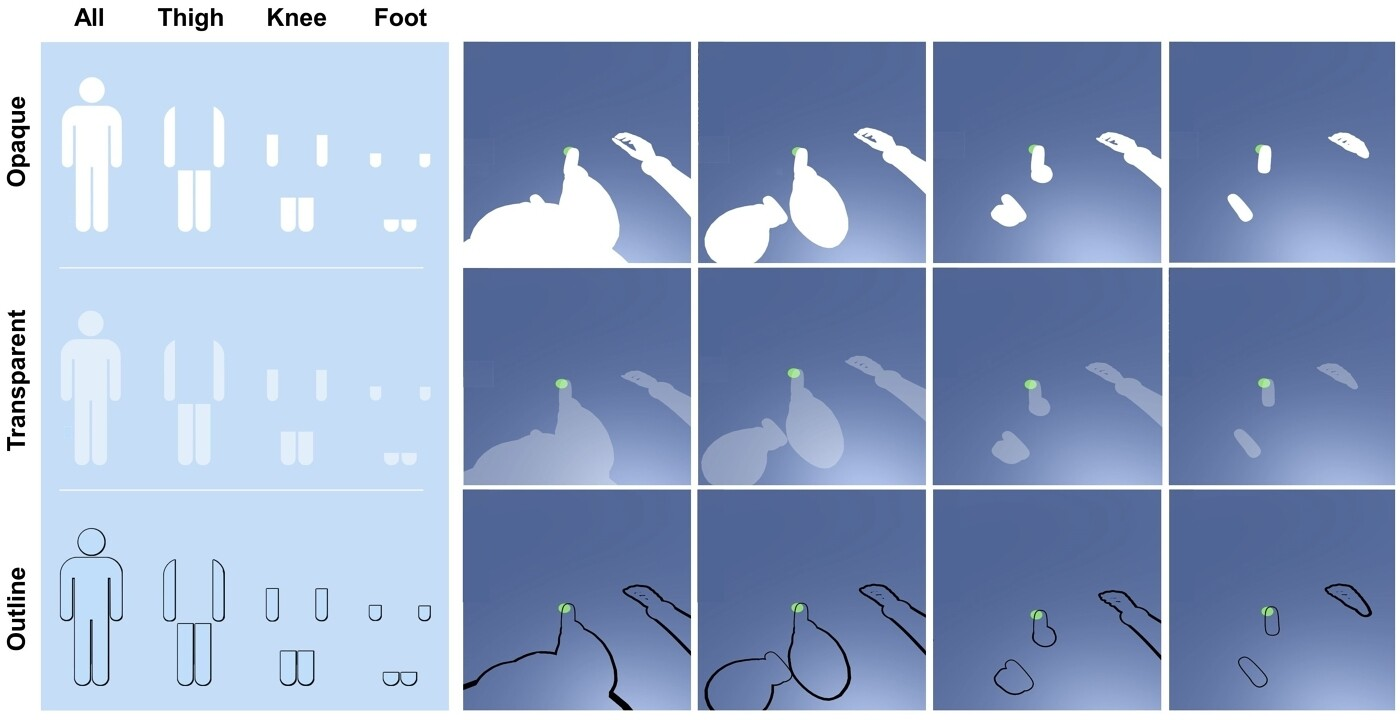
\includegraphics[width=0.8\linewidth]{fig/kanren1.jpg}
  \caption{SeeThroughBodyの各表示条件}
  \label{fig:1}
\end{figure}

評価実験では，身体の表示スタイルと表示部位を変更した際の影響を，客観的な操作性能と主観的なユーザ体験の両面から調査した．客観的な評価では，操作に要する時間や身体の移動量などを扱い，主観的な評価では，身体の存在感や使いやすさなどを調査している．このように，遮蔽が軽減されたかどうかだけでなく，表示方法の変更が操作時の体験にも与える影響を評価している．

実験の結果，身体の表示スタイルや表示部位の変更によって，遮蔽が軽減され，操作性能が改善することが示された．一方で，表示方法によって主観的なユーザ体験にも違いが生じ，操作性能とユーザ体験の間にトレードオフがあることが報告されている．具体的には，操作効率を重視する場合には足を透明にするTransparent-Footや，足の輪郭を表示するOutline-Footが推奨された．また，ユーザ体験全体を重視する場合には，全身を透明にするTransparent-Allや，大腿部を透明にするTransparent-Thighが推奨された．

同研究では，\figref{fig:2}に示すように得られた知見を足によるタッチ操作を用いた地図閲覧に適用し，身体の表示方法を変更する手法の応用例を示している．このように，VR空間において身体の表示方法を変更することは，遮蔽による操作上の問題を軽減するだけでなく，操作性能やユーザ体験にも影響することが示されている

\begin{figure}[htbp]
  \centering
  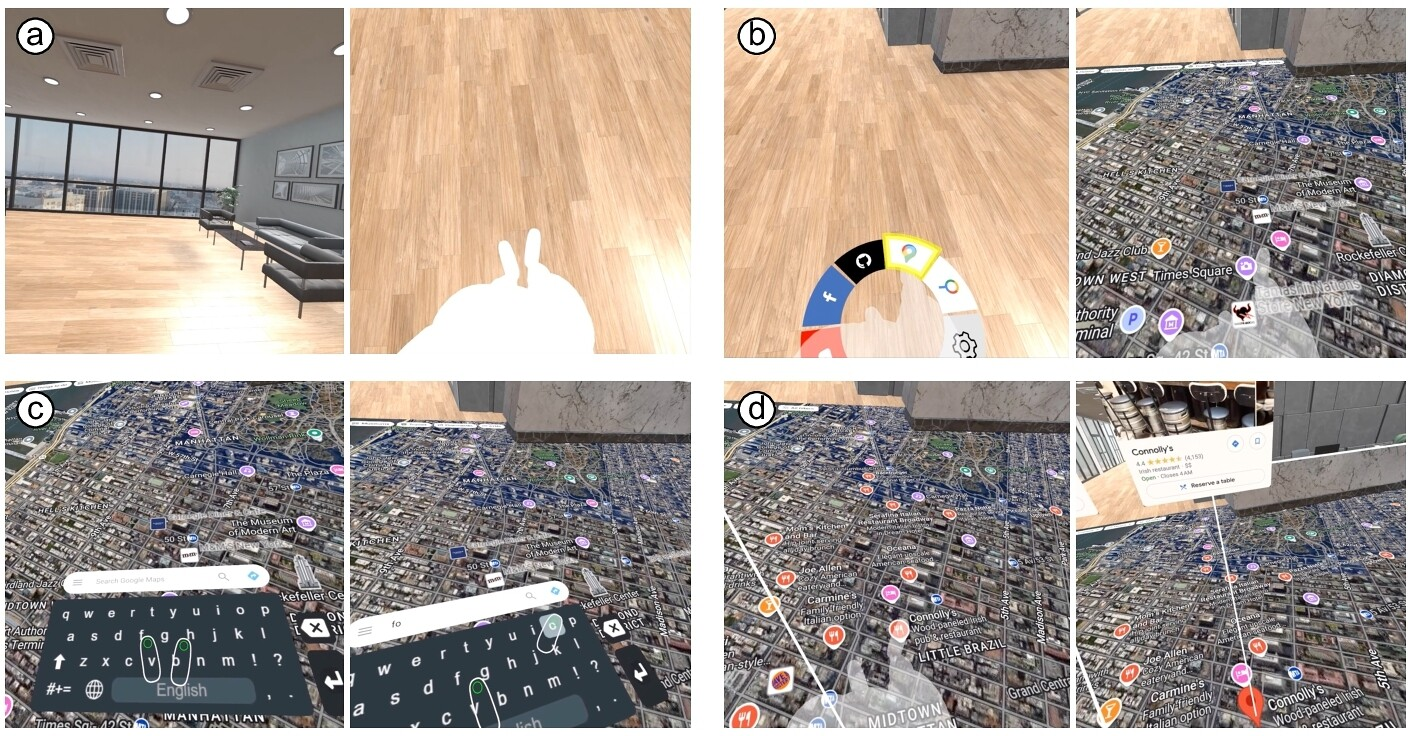
\includegraphics[width=0.8\linewidth]{fig/kanren2.jpg}
  \caption{足を用いた地図閲覧への適用例}
  \label{fig:2}
\end{figure}


一方，同研究は身体による遮蔽を対象としており，VRゲームにおける攻撃エフェクトによる遮蔽や，その表示方法がゲーム体験に及ぼす影響については検討されていない．

そこで本研究では，VRゲームにおけるブレス攻撃エフェクトに着目し，視認性を確保しながらゲーム体験を損なわない表示方法について検討する．